\section{Infrared Thermography}
\label{sec:sectiona}

Heat transfer through radiation is the way, in thermography, most often used to gather quantitative information on surface temperature. One of the main objectives of this work is to correctly convert the measured radiation intensity plus the information on the body emissivity and surrounding conditions in an accurate temperature estimate. To do so, some theoretical notions must be introduced.

\subsection{Radiation Intensity to Temperature Conversion}
\label{subsec:rad2tem}

Radiation is emitted by all bodies at $T>0 K$. The intensity of this radiation largely depends on the direction, wavelength and of course temperatures. For example, above 500ºC, a body's radiation is almost entirely in the IR wavelength \cite{IRCAM}. Besides emitting radiation a body can also absorb ($\alpha$), reflect ($\rho$) and radiation can even pass through it ($\tau$). Adding all this elements we get the Total Radiation Law:
\begin{equation}\label{eq:w}
    W = W\alpha + W\rho + W\tau
\end{equation}
in which $W$ represents the total energy transmitted through radiation. Equation \ref{eq:w} can be simplified as:
\begin{equation}\label{eq:1}
	1 = \alpha + \rho + \tau
\end{equation}
Note that in the equation \ref{eq:1}, $\alpha$, $\rho$ and $\tau$ represent the respective absorbed, reflected and transmitted fractions of the incident radiation energy, and have values between 0 and 1.\\

\subsubsection{Blackbody Equations}

\par One of the most important concepts that is used in this work is the concept of \textit{blackbody}. A \textit{blackbody} is characterized for absorbing all energy transmitted through radiation. In the ideal case of a \textit{blackbody} the coefficients assume the following values: $\alpha=1, \ \rho=0, \ \tau=0$. The blackbody is also a perfect emitter. The emissivity ($\varepsilon$) of a body characterizes the efficiency of a body for emitting energy, so it's the ratio between the energy emitted and the energy emitted if the body was a \textit{blackbody}. With this in mind one can use the equation \ref{eq:2} for a \textit{blackbody}. This equation is called Kirchhoff Law. Kirchhoff Law is also applied for the same wavelength ($\lambda$) so one can also use equation \ref{eq:3}.

\begin{equation}\label{eq:2}
\alpha=\varepsilon
\end{equation}
\begin{equation}\label{eq:3}
\alpha(\lambda)=\varepsilon(\lambda)
\end{equation}
\par For the specific case of a \textit{blackbody} one can also apply equation \ref{eq:4}. This equation is called Stefan-Boltzmann law and it states the relation between energy emitted through radiation and the temperature of the body. If the body is not perfectly black, but it's absorption/reflection/transparency properties don't vary with the wavelength, it's called as \textit{greybody} and in this case one should use Equation \ref{eq:5}.
\begin{equation}\label{eq:4}
W=\sigma_{SB} T^4
\end{equation}
\begin{equation}\label{eq:5}
W=\varepsilon \sigma_{SB} T^4
\end{equation}
where $\sigma_{SB}=5.670373 \times 10^8 W m^{-2} K^{-4}$ is the Stefan-Boltzmann constant.\\
\par It's fairly obvious these are concepts that illustrate ideal situations, and even though in most experiments shown further ahead the materials are chosen to be as close to \textit{black} or \textit{greybodies}, those aren't perfect. Of course this is attenuated by the fact that thermography measures in small intervals of wavelength. The next subsection will relate how a wavelength interval is selected, and it's relation with the atmosphere.

\subsubsection{Atmosphere Attenuation}
\label{subsec:atmat}

\par Almost every thermographical camera is separated from its target by the atmosphere, which has good or bad transmittance in different wavelengths. The atmosphere attenuation depends on the complexity of it's composition. For example, each of the following molecules: $H_2O$, $O_2$, $CO_2$ have certain wavelength values for which $\tau=0$. This means that in these wavelengths IR radiation will not pass through the atmosphere and its intensity cannot be measured.\\


\begin{figure}[h]
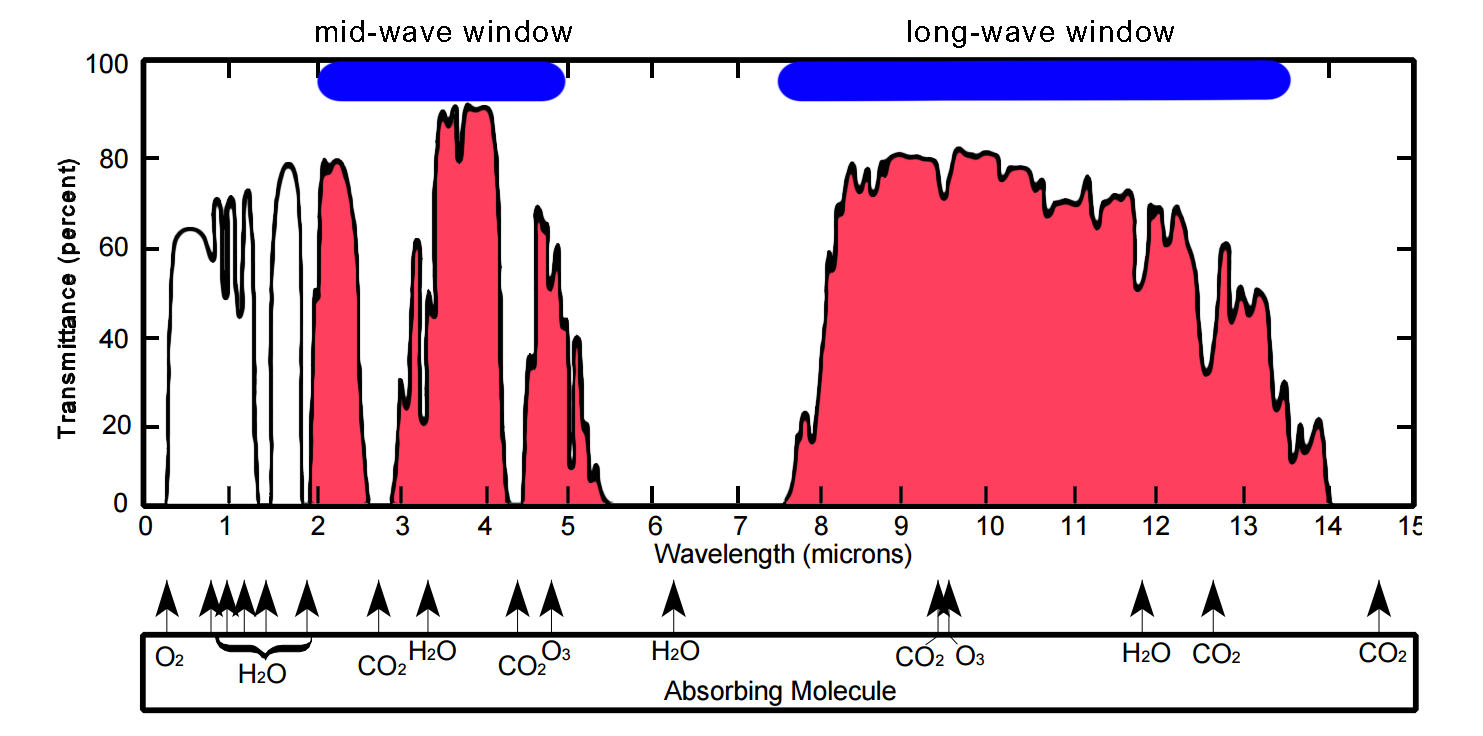
\includegraphics[width=1\linewidth]{Figures/2.Chapter/atmospheric_window.png}
\caption{Atmospheric Windows}
\source{Adaptation from chapter 7's Figure 10 of \cite{desk1997electronic}}
\label{fig:atm}
\end{figure}

\par This issue calls requires of choosing a wavelength \textit{window} for which the transmittance is close to 1. These \textit{windows} can be seen in Figure \ref{fig:atm}. It is possible to identify 2 main regions: the medium-wave \textit{window} (from 2-5 $m \mu$), or MW, and the long-wave \textit{window} (from 7.5-13.5 $m \mu$), or LW. The used camera works in the MW range so a selective range of wavelength inside it had to be chosen to avoid "bad atmosphere transmittance".\\

\subsubsection{Total Radiation}
\par When measuring a body's temperature with the IR Camera, there are other radiation sources that have to be accounted for. In total one can divide these radiation sources in 3 categories, shown bellow:
\begin{itemize}
\item The radiation emitted by the object/objects of study
\begin{equation}
W_{obj}=\varepsilon_{obj} \ \sigma_{SB} \ T_{obj}^4
\end{equation}
\item The radiation emitted by the atmosphere (where $ \ \varepsilon_{atm}=1-\tau_{atm}$ because $\rho_{atm}~=0$)
\begin{equation}
W_{atm}= (1-\tau_{atm}) \ \sigma_{SB} \ T_{atm}^4
\end{equation}
\item The radiation from the surroundings reflected by the object/objects.
\end{itemize}
\begin{equation}
W_{refl}=(1-\varepsilon_{obj}) \ \sigma_{SB} \ T_{refl}^4
\end{equation}
where $T_{refl}$ refers to the apparent temperature of the surroundings radiating to the measured body.\\
\par Figure \ref{fig:camscheme} identifies these sources and their origin. Note all the expressions in the figure represent energy radiated. In it it's possible to observe that 2 sources of radiation come from the studied body and represent the emitted and reflected components. When these components cross the atmosphere, they are affected by its transmissivity, $\tau_{atm}$ (this value in common atmospheric conditions is close to 1). The atmosphere itself can emit radiation, but because $\tau_{atm}$ is so close to 1, this is mostly negligible.\\

\begin{figure}
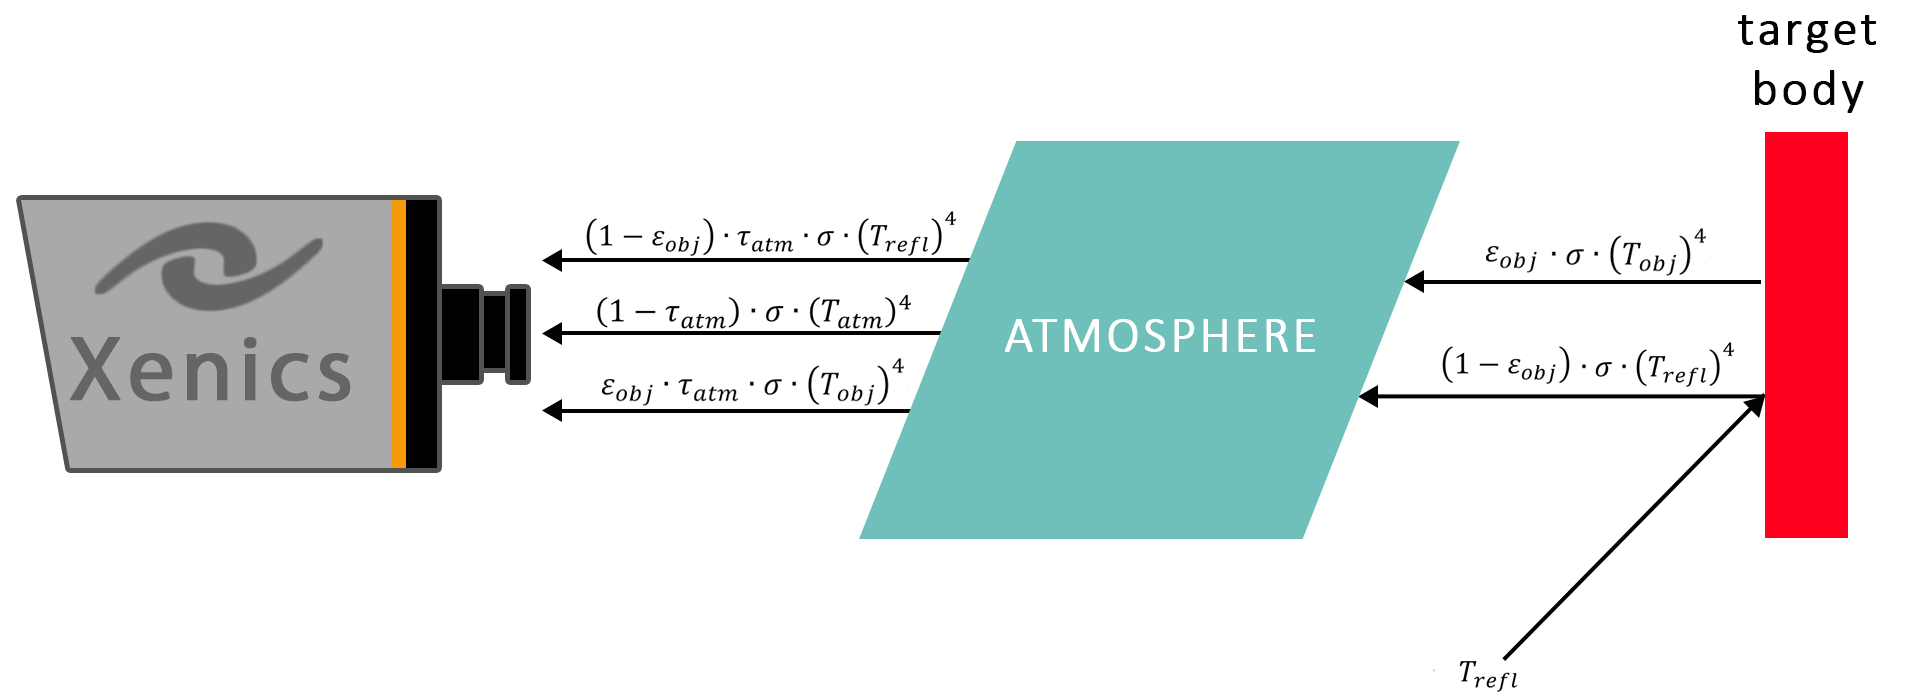
\includegraphics[width=1\linewidth]{Figures/2.Chapter/ir_camera_radiation_scheme.png}
\caption{Total radiation sources scheme}
\label{fig:camscheme}
\end{figure}

\par With these equations it is possible to relate the radiated energy received $W$ and the body temperature. This relation is seen in equations \ref{eq:6} and \ref{eq:7}.
\begin{equation}\label{eq:6}
W_{tot}=W_{obj}+W_{refl}+W_{atm}=(\varepsilon_{obj} \ \sigma_{SB} \ T_{obj}^4)+((1-\varepsilon_{obj}) \ \sigma_{SB} \ T_{refl}^4)+((1-\tau_{atm}) \ \sigma_{SB} \ T_{atm}^4)
\end{equation}
\begin{equation}\label{eq:7}
T_{obj}=\sqrt[4]{\frac{W_{tot}-(1-\varepsilon_{obj}) \ \sigma_{SB} \ T_{refl}^4-(1-\tau_{atm}) \ \sigma_{SB} \ T_{atm}^4}{\sigma_{SB} \ \varepsilon_{obj}}}
\end{equation}
\par The camera receives the total radiation $W_{tot}$, and the user has to input the emissivity and both the ambient and reflection temperatures in the camera software.

\section{Wettability}

\par Wettability is quantified by how well the surface is wetted by a liquid. This property is often characterized based on the equilibrium contact angle of a droplet deposited on a sold surface. This angle is given by the balance of the interface tensions acting between the surface, liquid and the vapor surroundings. The balance between these tensions is represented in Figure \ref{fig:tensao}
\begin{figure}[h]
\centering
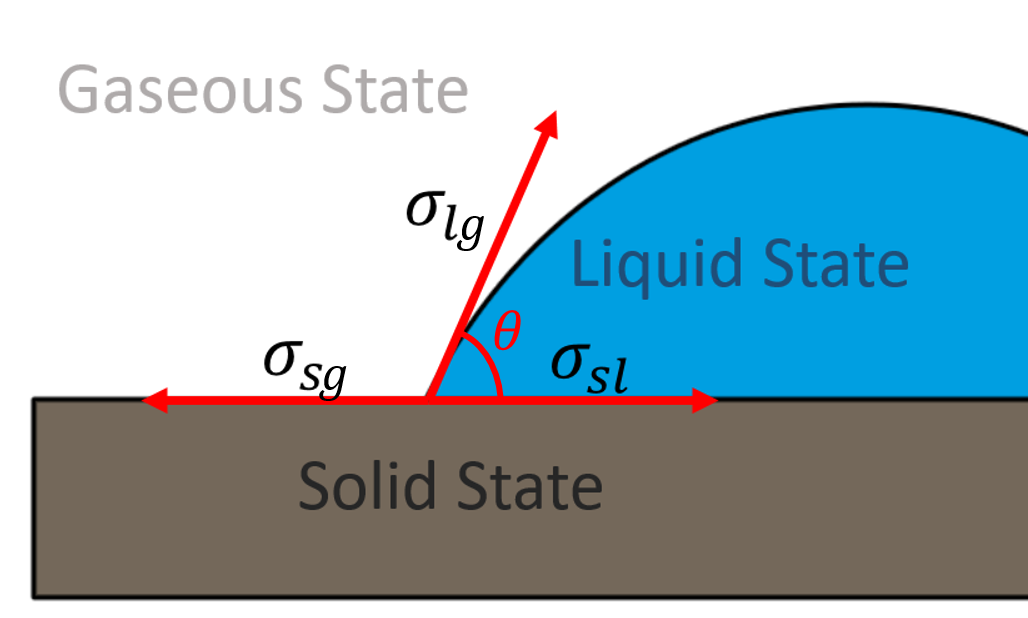
\includegraphics[width=0.5\linewidth]{Figures/2.Chapter/tensao.PNG}
\caption{Tension Balance}
\label{fig:tensao}
\end{figure}
\par From a thermodynamics perspective, the equilibrium condition of a liquid droplet are calculated by the minimization of the Gibbs energy of the system, G. When one considers constant temperature and pressure conditions it is possible to derive the well known Young's equation \cite{young1805essay} from this minimization ($dG=0$), which is simply the aforementioned balance of the interface tensions in the horizontal axis:
\begin{equation}
\sigma_{sg}=\sigma_{sl}+\sigma_{lg}cos(\theta_e)
\end{equation}
where $\sigma$ represents the interface tension at the solid-liquid (sl), solid-gaseous (sg) and liquid-gaseous (lg) boundaries and $\theta_e$ represents the equilibrium contact angle. High wettability droplet-surface-surrounding systems have $0\si{\degree} <\theta_e<90\si{\degree} $ and low wettability have $90\si{\degree}<\theta_e<180\si{\degree} $. The perfect wetted system has $\theta=0\si{\degree} $ and the perfect non-wetted system has $\theta=180\si{\degree} $ \cite{choi2011wettability}. If the liquid in study is water, the well wetted surfaces are called hydrophilic, while poor wetted surfaces are hydrophobic. Since ideal wetting/non-wetting situations do not exist, several authors (e.g. Koch \textit{et. al.} \cite{koch2009superhydrophobic}) consider the concept of superhydrophilic in $\theta_e<10\si{\degree}$ and superhydrophobic surfaces $\theta_e>150\si{\degree}$ the latter must also depict low histeresis. These regimes are depicted in Figure \ref{fig:wet}.

\begin{figure}[h]
\centering
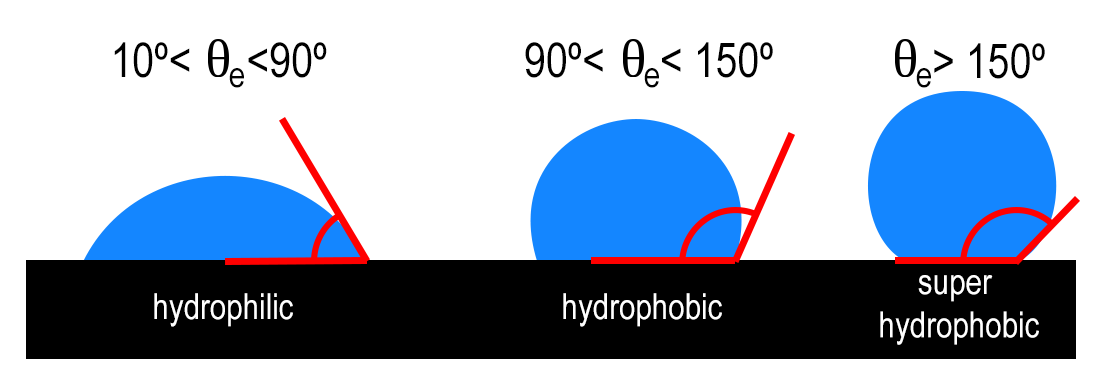
\includegraphics[width=0.7\linewidth]{Figures/2.Chapter/wet.png}
\caption{Wetting Regimes}
\label{fig:wet}
\end{figure}

\par While Young equation assumes that the surface is ideally smooth, in reality one has to take in account the roughness of the surface. Considering an rough homogeneous interface, one can convert the smooth surface contact angle ($\theta_e$) to the actual contact angle ($\theta$) using a formula based on the force balance and empirical correlations, presented in Equation \ref{eq:wenzel}. 
\begin{equation}\label{eq:wenzel}
cos \theta = R_f cos \theta_e
\end{equation}
where $R_f= \frac{A_{SL}}{A_{F}}$ is the relation between the surface area, to its flat projected area. This equation is called the Wenzel equation \cite{wenzel1936resistance}. Cassie took a different approach and considered an heterogeneous interface, where air would be trapped between the liquid and the surface, in pockets formed by the surface roughness. So having an interface with a fraction $f_1$ at one contact angle $\theta_1$ and another at $f_2$ and $\theta_2$, the contact angle would be given by Cassie's Equation \cite{cassie1944wettability} :
\begin{equation}\label{eq:cassie}
cos \theta = f_1 cos \theta_1 + f_2 cos \theta_2
\end{equation}
\par The difference between these two approaches can be seen in Figure \ref{fig:wenzelcassie}

\begin{figure}[h]
\centering
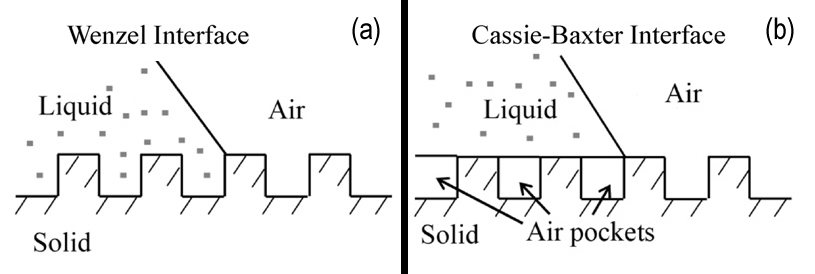
\includegraphics[width=0.7\linewidth]{Figures/2.Chapter/wenzelcassie.png}
\caption{Contact Angle approaches: (a) Wenzel, (b) Cassie-Baxter}
\source{Adapted from Bhushan, 2011\cite{bhushan2011natural}}
\label{fig:wenzelcassie}
\end{figure}


\section{Droplet Impact}

\par Several outcomes arrive from droplet impact, which depends on the impact conditions (size of the droplet and impact velocity), liquid properties and the boundary conditions established by the surface temperature and wettabillity:

\begin{itemize}
\item Rebound: after the impact the droplet bounces the surface partially or fully. Partial rebound happens when the surface is hydrophobic, while full rebound usually requires the surface to be super-hydrophobic.
\item Stick and Spread: the droplet sticks to the surface after the impact, spreading in the radial direction on the thin liquid film lamella. This is characteristic of hydrophilic surfaces.
\item Disintegration: the droplet sticks to the surface but smaller droplets are released in the spreading phase. Different disintegration mechanisms can be identified depending on the wettability, surface topography and impact conditions (Moita \textit{et. al.} \cite{moita2007drop}).
\end{itemize}

\par As the droplet hits the surface it deforms and spreads as a radial liquid film on the surface. The different outcomes arrive after this initial impact stage called as the kinematic phase.
As the liquid film (lamella) starts to form, the spreading velocity is dictated by the velocity of the contact edge of the film that instantly forms ($u_ce$). This parameter can be related with the droplet impact velocity($u_i$) and with the contact angle using \ref{eq:droplet}.
\begin{equation} \label{eq:droplet}
u_{ce}=\frac{u_i}{tan \theta}
\end{equation}

\par The lamella continues to spread governed by inertial effects until reaching its maximum diameter. Afterwards the lamella starts to recoil until reaching an equilibrium state.\\

\par While the earlier stages of spreading until reaching the maximum spreading diameter are governed by inertia, at the maximum spreading and at the recoiling phases viscous dissipation and wettability gain relative importance. Hence, spreading followed by recoiling is usually observed for impacts on hydrophilic surfaces, while rebound often occurs on hydrophobic surfaces, as the wettability precludes the contact between the lamella and the surface, lessening the viscous dissipation. Consequently, at the end of the recoiling phase the excess of surface energy is high enough to promote the droplet rebond from the surfaces. These phenomena are illustrated in figures 2.6 and 2.7.\\

\par To characterize the spreading and the recoiling phases many authors usually consider the spreading ratio $\beta(f) =\frac{D(t)}{d_0}$, which provides the temporal variation of the spreading diameter made non dimentional by the initial droplet diameter \cite{rein1993phenomena}. The time is also often made non dimensional as:

\begin{equation}\label{eq:rein}
t^*=\frac{t u_i}{r}
\end{equation}

where r is the droplet radius at that time.

\begin{figure}[h]
\centering
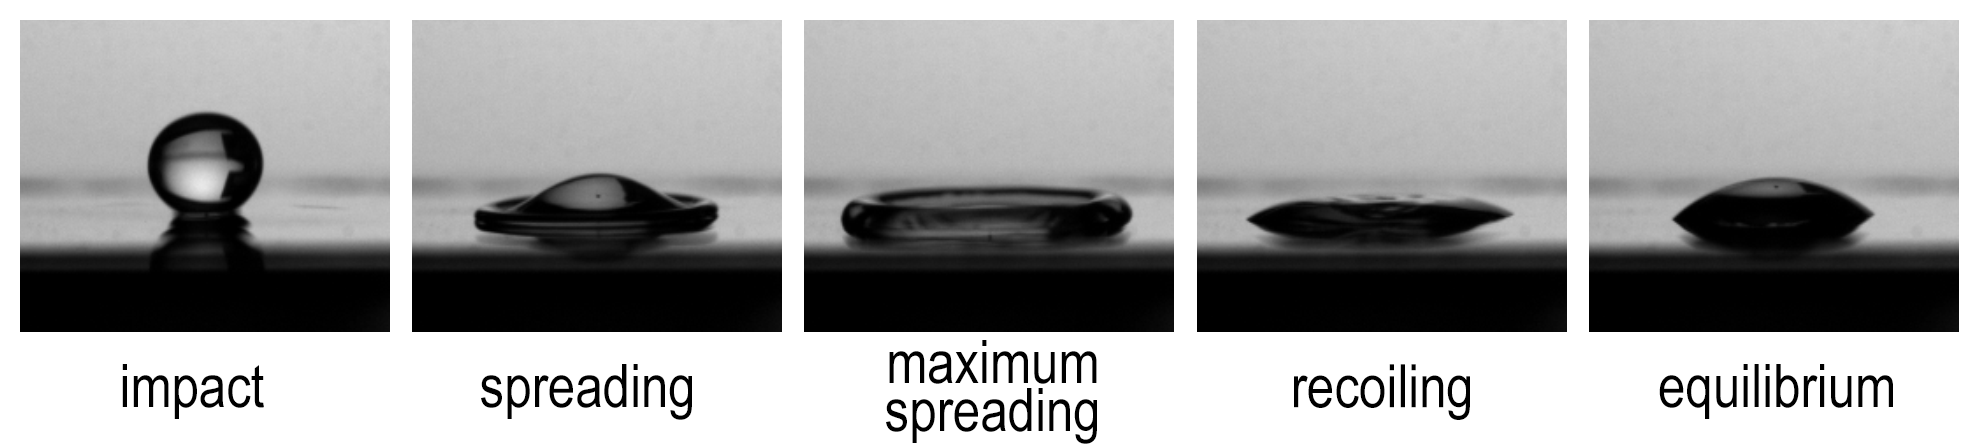
\includegraphics[width=0.9\linewidth]{Figures/2.Chapter/droplet.png}
\caption{Droplet impact stages, for an hydrophilic surface}
\label{fig:droplet}
\end{figure}

\begin{figure}[h]
\centering
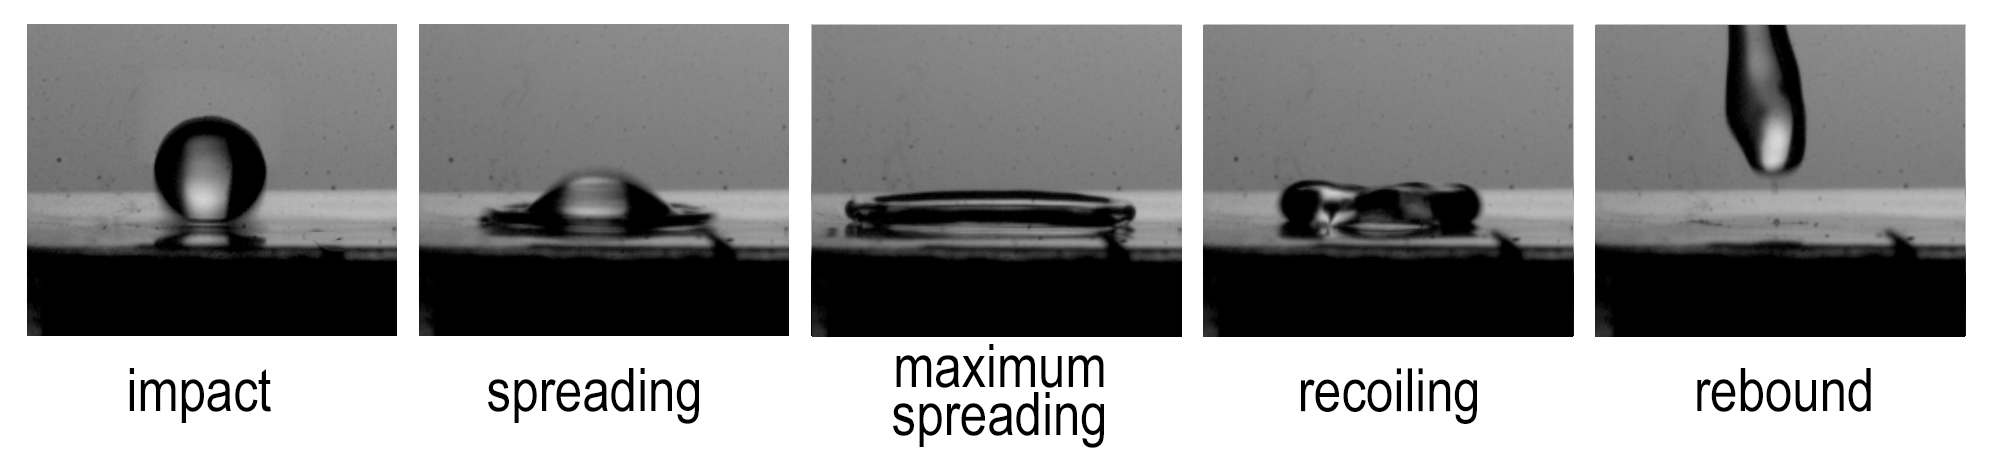
\includegraphics[width=0.9\linewidth]{Figures/2.Chapter/droplethf.png}
\caption{Droplet impact stages, for an hydrophobic surface}
\label{fig:droplethf}
\end{figure}

\section{Heat Transfer}
\label{sec:heat}

\par During droplet impact, the most important heat flux to evaluate is the change of heat between the droplet and the heater. According to \cite{sielaff2014experimental}, the heat flux from the droplet can be written as:

\begin{equation}\label{eq:heat}
q''=q_0''+k_h \delta (\frac{{\partial}^2 T}{\partial x^2}+\frac{{\partial}^2 T}{\partial y^2})-\rho_h c_{p,h} \delta \frac{{\partial} T}{\partial t} \quad [W/m^2]
\end{equation}

where $q_0$ is the heat flux from the heater, $k_h$, $\rho_h$ and $c_{p,h}$ are the conductivity, density and specific heat capacity of the heater's material and $\delta$ is the thickness of the heater. Across the radius of the droplet, the heat flux curves are similar to these reported by \cite{pasandideh2001cooling} and represented in Figure \ref{fig:fluxo}. High heat transfer occurs in the first instants after impact (t< 2 ms). As the droplet spreads a peak in the heat flux is observed at the edge of the lamela. This is due to "new" cold liquid reaching the hot surface. The heat flux is reduced substantially in time at later stages of spreading (t>4 ms), mainly because the droplet is heating and the liquid speed is decelerating, thus reducing convective and conductive heat transfer.

\begin{figure}[h]
\centering
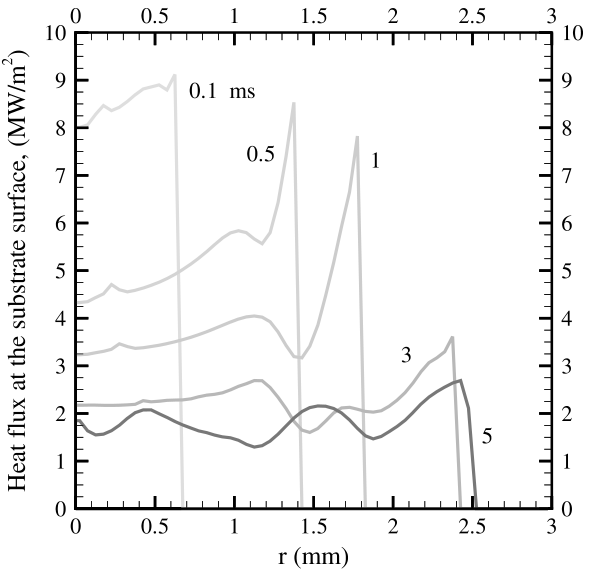
\includegraphics[width=0.5\linewidth]{Figures/2.Chapter/fluxo.png}
\caption {Heat Flux at the surface for different timesteps}
\label{fig:fluxo}
\source{M. Pasandideh-Fard, 2001 \cite{pasandideh2001cooling}}
\end{figure}

\par In the droplet case, the flux for various points along the radius is being analyzed, and this calculation is made using cylindrical coordinates and considering the temperature distribution to be axyssimetrical. To convert the coordinate system, one should first consider the following transformation of the second derivative:

\begin{equation}
\frac{\partial^2}{\partial x^2}=(cos \phi \frac{\partial}{\partial r} - \frac{sin \phi}{r}\frac{\partial}{\partial \phi})(cos \phi \frac{\partial}{\partial r} - \frac{sin \phi}{r}\frac{\partial}{\partial \phi})
\end{equation}

\begin{equation}
\frac{\partial^2}{\partial y^2}=(sin \phi \frac{\partial}{\partial r} - \frac{cos \phi}{r}\frac{\partial}{\partial \phi})(sin \phi \frac{\partial}{\partial r} - \frac{cos \phi}{r}\frac{\partial}{\partial \phi})
\end{equation}

\par Considering now the condition of axyssimetry ( $\frac{\partial}{\partial \phi}=0$), and applying the expression to the temperature field, one can write the sum of the second derivatives as:

\begin{equation} \label{eq:coord}
\frac{\partial^2 T}{\partial x^2}+\frac{\partial^2 T}{\partial y^2}=(cos^2 \phi \frac{\partial^2 T}{\partial r^2}) + (sin^2 \phi \frac{\partial^2 T}{\partial r^2})= (cos^2 \phi + sin^2 \phi )\frac{\partial^2 T}{\partial r^2} = \frac{\partial^2 T}{\partial r^2}
\end{equation}

\par Thus, the equation for the heat flux removed by the droplet, considering the axyssimetry condition, can be written as:

\begin{equation}\label{eq:heatf}
q''=q_0''+k_h \delta (\frac{{\partial}^2 T}{\partial r^2})-\rho_h c_{p,h} \delta \frac{{\partial} T}{\partial t} \quad [W/m^2]
\end{equation}

\par The power dissipated ($P_{diss}$) by the droplet is the integral of this expression in the droplet area, and it's given by:

\begin{equation}\label{eq:diss}
P_{diss}= \int_{A} q'' \; dA \quad [W]
\end{equation}

\par Since the droplet, ideally, is always axisymetric, it is necessary to decompose $dA$ in cylindrical coordinates. Equation \ref{eq:diss} is expressed in cylindrical coordinates in Equation \ref{eq:cyl}. Integrating the power in time one ends up with the total heat extracted. This is expressed in Equation \ref{eq:qtot}.

\begin{equation} \label{eq:cyl}
P_{diss} = \int_\theta \int_r r \, q'' \; dr d\phi \quad [W]
\end{equation}
\begin{equation} \label{eq:qtot}
Q_{tot} = \int_t P_{diss} \; dt [J]
\end{equation}

\par Pasandideh-Fard \cite{pasandideh2001cooling} proposed a way to quantify the "cooling effectiveness" ($\epsilon$) of the droplet. This effectiveness is described by the actual heat removed by the droplet divided by the maximum heat transfer possible be removed in theory (assuming no phase change). This coefficient is described by Equation \ref{eq:epsilon}.

\begin{equation}\label{eq:epsilon}
\epsilon= \frac{\int_t \int_A q'' \; dA \, dt}{(m c_p \Delta T)_{water}}
\end{equation}

\par The relation between the cooling effectiveness and the time adimensionalized for different impact velocities has been computed by \cite{pasandideh2001cooling} and is shown in Figure \ref{fig:cooling}. The cooling effectiveness grows with the impact velocity because, as shown in Equation \ref{eq:rein}, the spreading factor is larger, meaning that the area covered by the droplet also grows.

\begin{figure}[h]
\centering
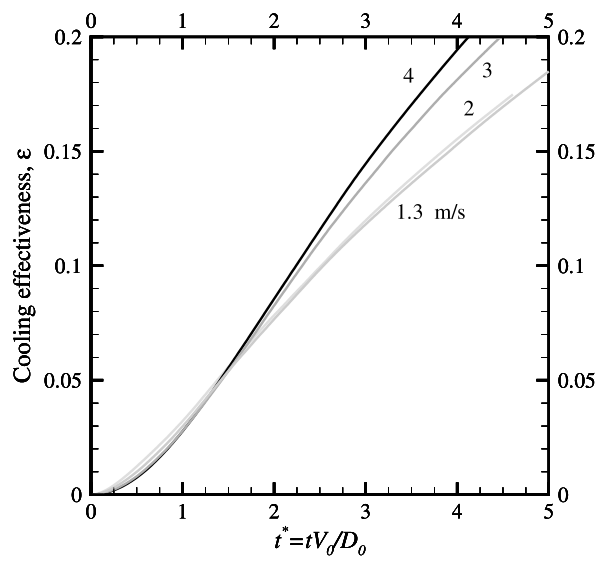
\includegraphics[width=0.5\linewidth]{Figures/2.Chapter/cooling.png}
\caption {Evolution of the calculated cooling effectiveness during the impact of a droplet on a surface initially at 120ºC}
\label{fig:cooling}
\source{M. Pasandideh-Fard, 2001 \cite{pasandideh2001cooling}}
\end{figure}

\par The heat transfer occurring during droplet spreading has particular complex characteristics as described in the literature (e.g. \cite{strotos2011non}). Figure \ref{fig:tempvar} illustrates approximately how the temperature of the surface evolves along the radius during droplet spreading. In the center of the droplet a bubble trapping effect creates a barrier for heat transfer, causing the temperature to have a slightly higher value. Also in the minimum thickness area the temperature is higher because the layer of liquid is thinner, removing less heat. In the contact edge, called rim, the liquid flowing from the lamella arrives and recirculates, so the temperature decreases again in this regime. The temperature raise at the end of the droplet, after the rim is naturally due to heat conduction from the heater within a region that is no longer wetted by the fluid.\\

\begin{figure}[h]
\centering
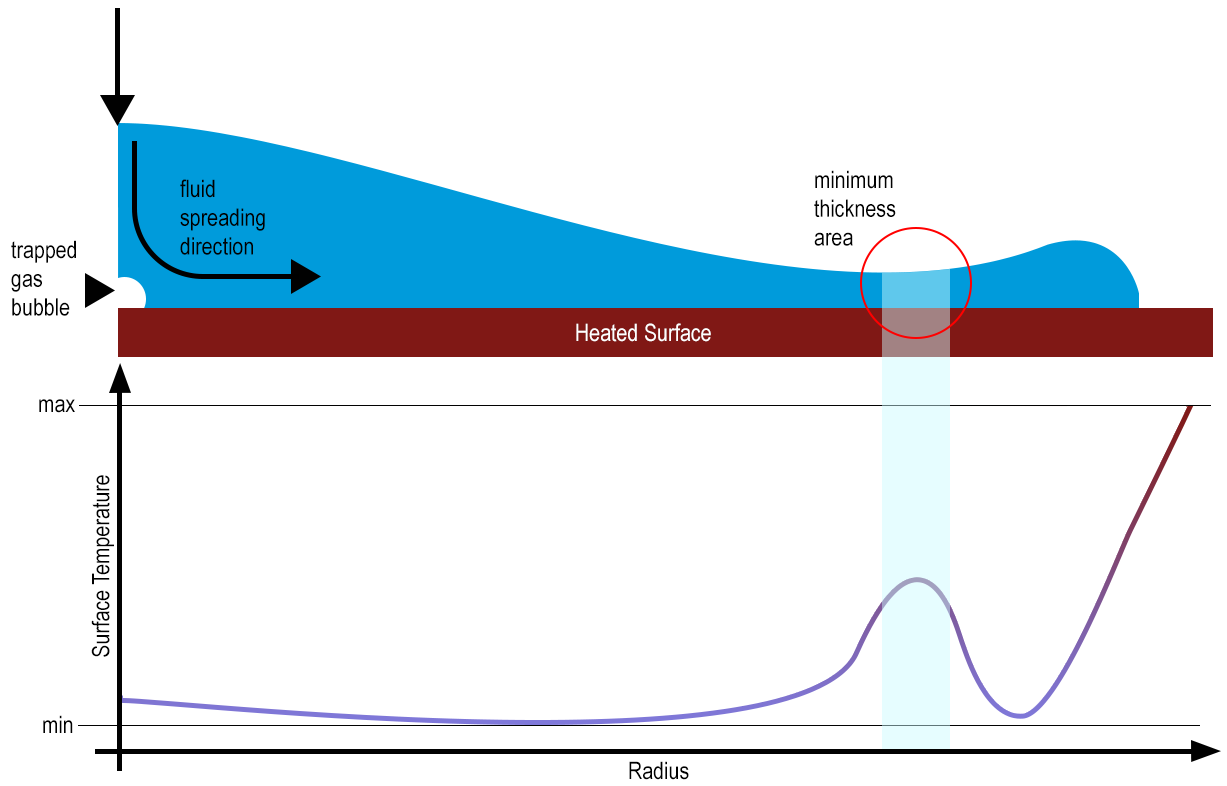
\includegraphics[width=1\linewidth]{Figures/2.Chapter/tempvar.png}
\caption {Scheme of the surface temperature variation along the droplet radius, during spreading}
\label{fig:tempvar}
\end{figure}


